\newpage
\section{Questão:12-31}

\begin{figure}[H]
	\centering
	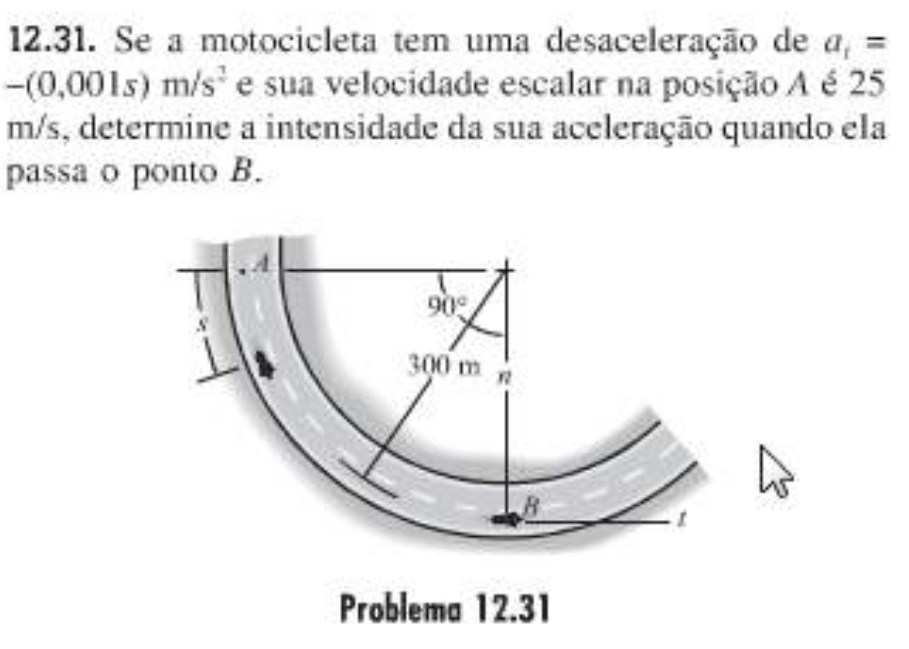
\includegraphics[width=.7\linewidth]{fundamentais/12-31.png}
	\caption{Comando da questão 12-31}\label{fig:12-31}
\end{figure}


Nesta questão, analisamos o movimento de uma partícula ao longo de uma curva circular com raio \(r = 300 \, \text{m}\). A aceleração tangencial da partícula é variável e descrita pela equação \(a_t = -0.001 \cdot s\), onde \(s\) é a posição ao longo do arco em metros. Sabemos que a velocidade da partícula no ponto \(A\) (\(s = 0\)) é \(v_A = 25 \, \text{m/s}\). Nosso objetivo é determinar a velocidade da partícula no ponto \(B\) (\(s = r = 300 \, \text{m}\)).

\subsection*{Equação do Movimento}
A equação do movimento é dada por:
\[
a_t = v \cdot \frac{dv}{ds},
\]
onde:
\begin{itemize}
    \item \(a_t = -0.001 \cdot s\): Aceleração tangencial variável;
    \item \(v\): Velocidade escalar da partícula;
    \item A distância percorrida \(s_B\) é: \( s_B = \rho \cdot \theta = 300\cdot \frac{pi}{2} = 471.24\, m\)
    
    \item \(s\): Posição ao longo do arco.
\end{itemize}

Substituímos \(a_t\) na equação:
\[
-0.001 \cdot s = v \cdot \frac{dv}{ds}.
\]

Reorganizando:
\[
v \cdot dv = -0.001 \cdot s \cdot ds.
\]

\subsection*{Integração}
Integramos ambos os lados para determinar \(v\) em função de \(s\). No ponto \(A\), temos \(v = v_A = 25 \, \text{m/s}\) quando \(s = 0\):
\[
\int_{v_A}^{v} v \, dv = \int_{0}^{s} -0.001 \cdot s \, ds.
\]

Resolvendo a integral do lado esquerdo:
\[
\frac{v^2}{2} \bigg|_{v_A}^{v} = -0.001 \cdot \frac{s^2}{2} \bigg|_{0}^{s}.
\]

Substituímos os limites:
\[
\frac{v^2}{2} - \frac{v_A^2}{2} = -0.001 \cdot \frac{s^2}{2}.
\]

Reorganizando para \(v^2\):
\[
v^2 = v_A^2 - 0.001 \cdot s^2.
\]

\subsection*{Velocidade no Ponto \(B\)}
No ponto \(B\), substituímos \(s = 471.24 \, \text{m}\) e \(v_A = 25 \, \text{m/s}\) na equação:
\[
v^2 = 25^2 - 0.001 \cdot (471.24)^2.
\]

Calculando:
\[
v^2 = 625 - 222,0671376.
\]

\[
v^2 = 402.933 \, m^2/s^2
\]

A velocidade no ponto \(B\) é:
\[
v = \sqrt{402.933} \approx 20.073 \, \text{m/s}.
\]

\subsection*{Resultado Final}
A velocidade da partícula no ponto \(B\) (\(s = r = 471.24 \, \text{m}\)) é:
\[
v \approx 20.073 \, \text{m/s}.
\]
